\chapter{Orchestration des applications distribuées}
\begin{onehalfspace}

\initial{D}ocker est un outil qui a révolutionné le monde informatique par l'introduction de la notion de conteneur, donc il est normal de chercher à l'utiliser en production. De nos jours, les développeurs utilisent de plus en plus Docker pour déployer des applications qui s’exécutent sur plusieurs conteneurs et plusieurs hôtes. Orchestrer ces applications distribuées nécessite une approche \textbf{multi-conteneur} et \textbf{multi-hôte} native avec une interface utilisateur et de l'outillage commun qui fonctionnent sur toutes les infrastructures. Plusieurs outils ont été présentés par de grandes entreprises et qui sont toujours en cours de développement. Nous exposerons dans ce chapitre les projets promoteurs dans l'orchestration des applications distribuées.

\newpage

\section{Le Clustering}

Nous avons présenté dans le chapitre 2 le Cloud Computing ainsi que ses services classiques. Dans cette section, nous allons parler du cluster comme un service et le situer dans le pyramide des services du Cloud (Figure ~\ref{fig:pyramide-cluster}).

\begin{figure}[H]
\centering
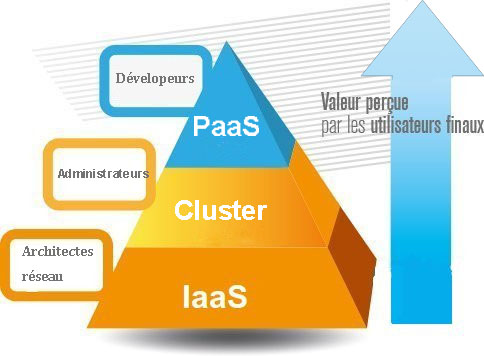
\includegraphics [scale=0.7]{chapitre3/assets/pyramide}
\caption{Le Cluster dans le Cloud}
\label{fig:pyramide-cluster}
\end{figure}

\begin{itemize}
	\item \textbf{Plate-forme}: Un développeur crée une application dans un ensemble particulier de langages de programmation à l'aide des \acrshort{api}s spécifiques et pousse ce code vers la plate-forme. La plate-forme l'exécute et lance une seule copie du service ou éventuellement plusieurs copies dépendamment du trafic. Finalement ce service monte en charge automatiquement. 
	\item \textbf{\acrshort{iaas}}: A l'autre bout du pyramide se trouve l'\acrshort{iaas} composé seulement de machines virtuelles qui résident essentiellement dans l'internet. Quand un utilisateur consulte un fournisseur \acrshort{iaas} et demande  un ordinateur avec des spécifications données (quantité de mémoire et de disque, nombre de \acrshort{cpu}, une version spécifique Linux, etc). En quelques minutes, L'utilisateur pourra  exécuter n'importe quel logiciel sur le serveur mais il est entièrement responsable de la gestion de la machine.
	\item \textbf{Cluster}: C'est lorsqu'il y a un besoin de gérer un ensemble de machines, un cluster de machines comme une seule entité, pas seulement un ordinateur individuel (\acrshort{iaas}) et non plus toute une plate-forme magique.

\end{itemize}


\def\arraystretch{1.6}%  1 is the default, change whatever you need

{\rowcolors{1}{tabOdd}{tabEven}
\begin{center}
\begin{table}[H]

	\begin{tabu}{| X[c] | X[c] | X[c] | X[c] |} 


	\hline
	\rowcolor{tabHead}
	\textbf{} & \textbf{IaaS (VMs)} & \textbf{Cluster} & \textbf{Plate-forme}\\ [0.95ex] 
	\hline\hline
	A quoi sert ? 	& Créer et déployer les images des machines virtuels & Créer et déployer des conteneurs & créer et déployer des applications (services) \\ 
	Automatise					& - & Ordonnancement & Tout \\ 
	gére					& Un seul atome & Des serveurs & Des applications \\ 
	fléxibilité					& ++ 	& + 	& - \\ 
	Agilité						& - 	& + 	& ++ \\ 
	\hline
	\end{tabu}
	\caption{Le Cluster dans le Cloud}
	\label{tab:table_label}

\end{table}
\end{center}
}


En général, un cluster comporte plusieurs éléments qu'on définit ci-dessous :

\begin{itemize}
	\item \textbf{Master} : C'est la machine qui est responsable du Cluster. Il veille sur son bon fonctionnement grâce au système de découverte des services et l'ordonnanceur
	\item \textbf{Ordonnanceur} : Dans un ordinateur ordinaire, pour démarrer un processus, on a besoin d'un gestionnaire des processus pour les faire fonctionner et les garder en cours d'exécution. L'ordonnanceur le fera sur l'ensemble des machines (Cluster)
	\item \textbf{Nœud} : Une machine qui appartient au Cluster, elle peut être réelle ou virtuelle.
	\item \textbf{Gestionnaire des conteneurs} : C'est la partie de logiciel qui est distribuée dans chaque machine du cluster. Il supervise les conteneurs ordonnancés, les redémarrent en cas de nécessité.
	\item \textbf{Conteneurs ordonnancés} : Un service fonctionne à l'intérieur d'un conteneur ordonnancé. En effet, ce conteneur se trouve dans une telle machine  parce que le développeur a déclaré à l'ordonnanceur du Cluster (maître) les besoins du service en terme de ressources (nombre de CPU, RAM, etc...). L'ordonnanceur fournit pour le service un endroit où il peut vivre en paix.
\end{itemize}


\begin{figure}[H]
\centering
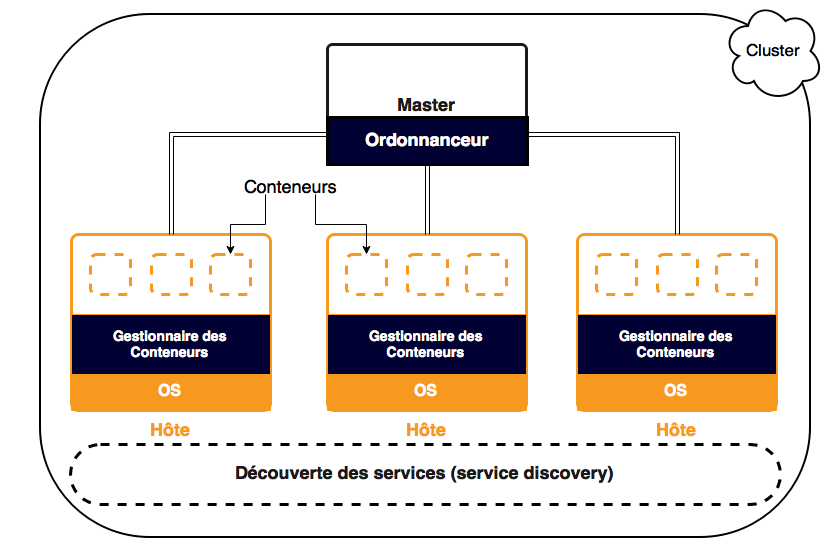
\includegraphics [scale=0.55]{chapitre3/assets/cluster}
\caption{Un cluster en général}
\label{fig:}
\end{figure}

Nous avons vu la notion de cluster et les processus d'automatisation et coordination. De ce fait, la gestion des services informatiques distribués se trouve incontournable au fonctionnement du cluster, elle est appelé \textbf{l'orchestration}. Dans la section suivante, nous allons détailler les différents solutions d'orchestration qui existent dans le monde de la containérisation.

\section{Orchestration Docker}
Les capacités d'orchestration de Docker sont construites sur les fondations existante de Docker. Ces capacités sont assurées par trois nouveaux services de la plate-forme qui sont conçus pour couvrir tous les aspects du cycle de vie dynamique des applications distribuées. Selon l'entreprise Docker, toutes ces caractéristiques sont conçues avec la philosophie de conception "\emph{Batteries Included, but Removable}" qui indique qu'ils peuvent fonctionner avec des services tierces. Ceci offre le choix aux clients de choisir entre les différents outils d'orchestration de Docker et les alternatives communautaires.


%\begin{figure}[H]
%\centering
%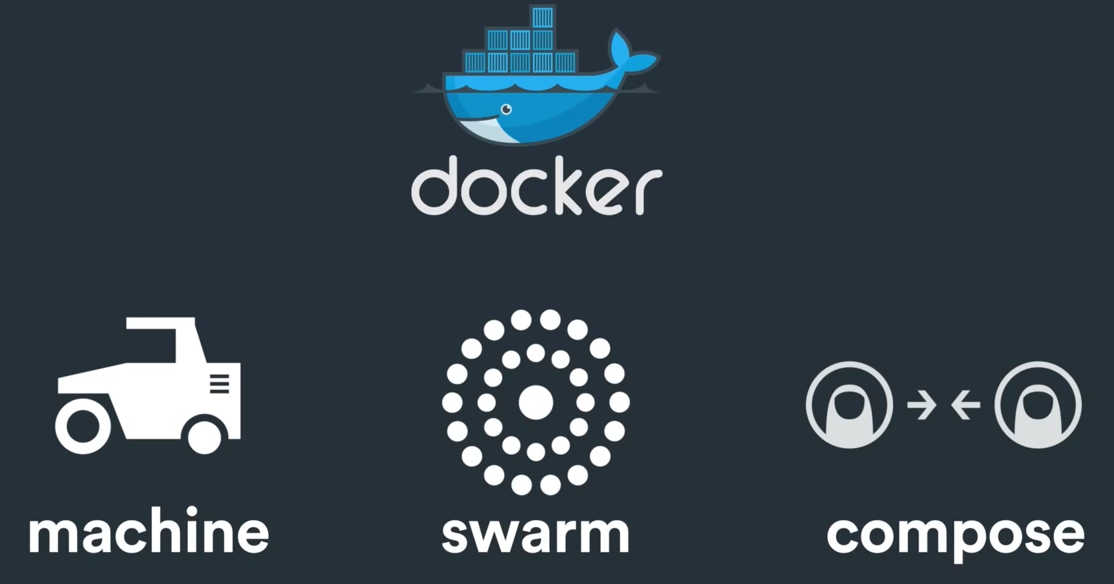
\includegraphics [scale=0.4]{chapitre3/assets/orchestrationdocker.png}
%\caption{Orchestration Docker}
%\end{figure}
\subsection*{Docker Machine}
 Ce service facilite le provisionnement d'un hôte avec Docker installé dans une variété d'environnements. Les développeurs peuvent rapidement lancer les machines hôtes exécutant Docker ; sur un ordinateur portable, un Datacenter de VMs, ou une instance Cloud. Cela évite la tâche de se connecter à un hôte pour installer et configurer le démon Docker et le client. Bien que toujours en version alpha, Docker machine prend en charge le provisionning de Docker localement avec VirtualBox et à distance sur les instances Digital Ocean. Le support pour AWS, Azure, VMware, OpenStack et d'autres infrastructures devrait arriver rapidement.
 \begin{figure}[H]
\centering
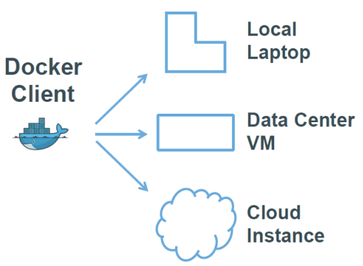
\includegraphics [scale=0.6]{chapitre3/assets/dockermachine.png}
\caption{Docker Machine}
\end{figure}
\subsection*{Docker Swarm}
 Docker Swarm est un service de Clustering natif de Docker qui fonctionne avec l'engine Docker standard, et qui crée un pool de ressources sur lesquels les applications distribuées s'exécutent. Cela permet aux développeurs et équipes opérationnelles de considérer un cluster de machines Docker comme un pool de ressources unique. Les administrateurs peuvent planifier des conteneurs qui seront lancés dans l'un des hôtes qui répond aux exigences. Docker Swarm fournit des contraintes standard et personnalisées pour répondre aux besoins et à la planification basée sur des règles, cela permet de déclarer des exigences et contraintes spécifiques à chaque conteneur. Docker Swarm est conçu pour évoluer avec le cycle de vie de l'application. Il peut prendre en charge un hôte dans l'environnement de développement et d'autres s'exécutant dans l'environnement de production.
\begin{figure}[H]
\centering
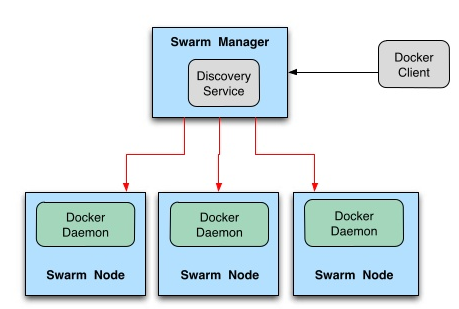
\includegraphics [scale=0.6]{chapitre3/assets/dockerswarm.png}
\caption{Architecture de Docker Swarm}
\end{figure}
\subsection*{Docker Compose}
  Docker Composer permet aux développeurs d'assembler des applications de conteneurs autonomes, interopérables et indépendants de l'infrastructure sous-jacente. Avec cette approche déclarative, il est facile de définir des stacks qui sont portables. Une stack d'applications distribuées est déclarée à travers un simple fichier de configuration \acrshort{yaml} qui contient la définition de chaque conteneur.
\begin{figure}[H]
\centering
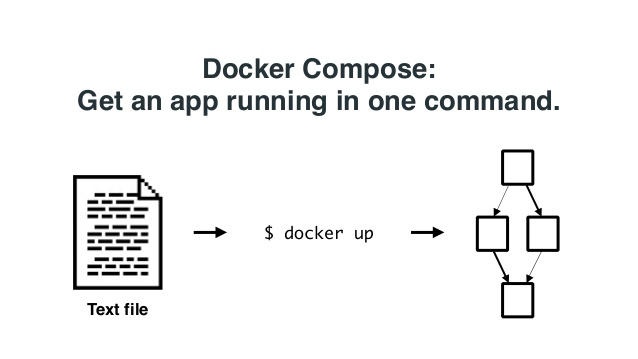
\includegraphics [scale=0.5]{chapitre3/assets/dockercompose.jpg}
\caption{Docker Compose}
\end{figure}
\section{Orchestration Google}
L'entreprise Google est aussi intéressée par l'orchestration des conteneurs docker, elle a d'ailleurs lancée un projet nommée \textbf{Kubernetes}.Ce projet est récent mais promoteur et pourrait révolutionner le domaine du Cloud s'il est suffisamment mature pour la production. Kubernetes a pour objectif de fournir un outil de supervision unique capable de déplacer des conteneurs Docker d'un Cloud à un autre. Autrement dit, de proposer une forme d’interopérabilité dans le nuage, via un framework de gestion de conteneurs solide, ouvert et adapté à toute application sur tous types d’environnements, qu’il s’agisse de Cloud privé, public ou hybride. Ce projet a le soutien et l'attention des géants du Cloud notamment Microsoft, IBM, RedHat qui tiennent à s'assurer que cet outil sera compatible avec leurs Clouds et tentent de l'associer au projet \textbf{Openstack} qui est l'orchestrateur du cloud hybride open source.
\subsection{Architecture de Kubernetes}
Kubernetes est un outil open-source pour l'orchestration des conteneurs Docker. Il gère l'ordonnancement des nœuds dans un Cluster et gère les ressources pour mieux correspondre à l'intention de l'utilisateur. En utilisant les concepts de "\emph{labels}" et "\emph{pods}", il permet un regroupement optimal de conteneurs pour une meilleure gestion et une découverte facile.
\begin{figure}[H]
\centering
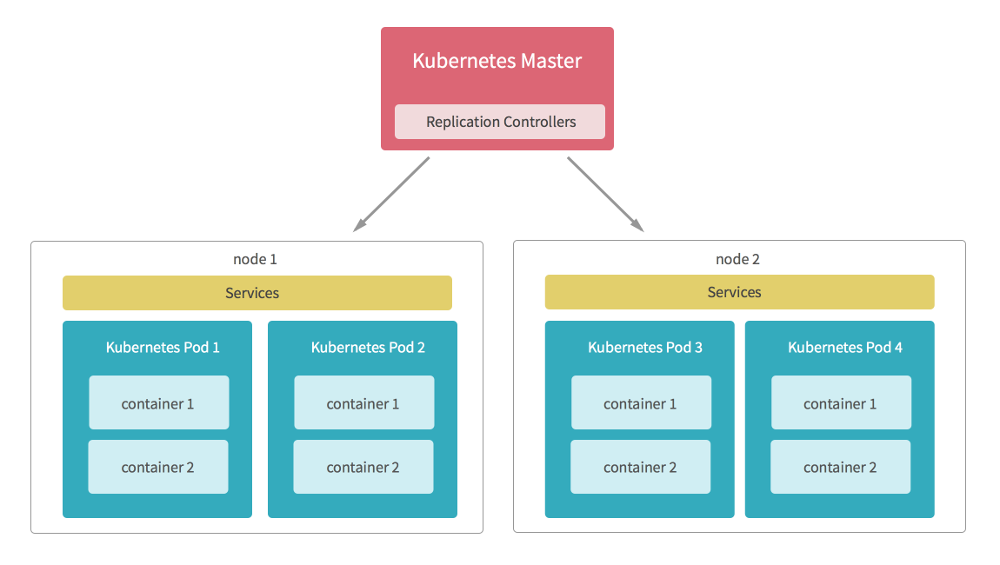
\includegraphics [scale=0.4]{chapitre3/assets/archkuber.png}
\caption{Architecture de Kubernetes}
\end{figure}

\begin{itemize}
\item \textbf{Kubernetes Master} : il contrôle l'ensemble du Cluster et exécute l'API. Fondamentalement, il est responsable du Cluster.

\item \textbf{Nodes} : un nœud est un serveur physique (ou une machine virtuelle) à l'intérieur du cluster. Il communique avec les maîtres et contient des conteneurs, on peut ajouter ou supprimer des nœuds à volonté.

\item \textbf{Pods} : un "\emph{Pod}" est le bloque basique de construction dans \emph{Kubernetes}.Dans un pod, il est possible de lancer plusieurs conteneurs. L'allocation des CPU, mémoire et des autres ressources est gérée dans un pod. Chaque pod possède sa propre adresse ip et son nom d'hôte pour éviter d'éventuels conflits de ports.

\item \textbf{Replication Controller} : Il est vrai que le Pod est un composant puissant au sein de \emph{Kubernetes} mais il ne permet pas la gestion des échecs. Les échecs sont des événements inévitables bien qu'il faudrait que le service soit toujours disponible. C'est de ce fait qu'intervient \emph{Replication Controller}. Ce dernier s'assure qu'un nombre donné de pods sont exécutés au sein du Cluster, il peut enlever et ajouter des pod du Cluster donc il faudra définir un pod template pour assurer sa fonction.

\item \textbf{Services} : les Pods sont ajoutés ou supprimés donc il faudrait permettre un \textbf{load-balancing} du trafic dans ses pods. "\emph{Service}" agit comme un \emph{load-balancer} dynamique pour un ensemble de pods, il est très efficace et utilise différentes techniques ( IP Tables, ...) pour éviter la surcharge.

\end{itemize}
%\begin{figure}[H]
%\centering
%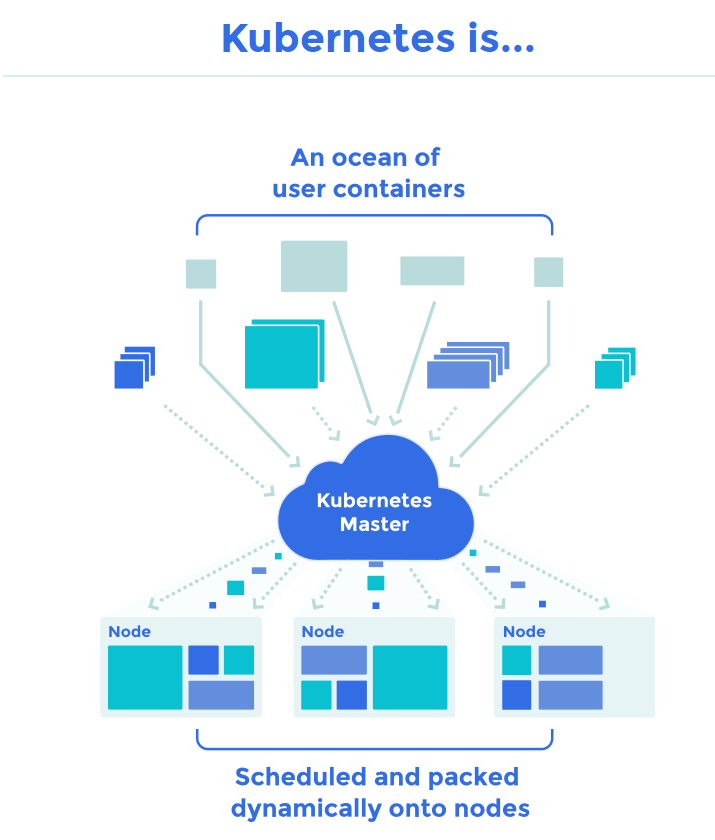
\includegraphics [scale=0.5]{chapitre3/assets/kuber.png}
%\caption{Résumé de Kubernetes}
%\end{figure}

\section{Orchestration Apache}
L'entreprise Apache a toujours été intéressée par le domaine du Cloud, le lancement de son projet \textbf{Mesos} visait principalement à améliorer l'orchestration des \emph{"datacenters"} ceci bien avant l’émergence des conteneurs et docker. Le projet Mesos est très promoteur pour le futur avec les conteneurs bien qu'il soit déjà mature avec les machines virtuelles. Plusieurs grandes entreprise utilisent Mesos notamment \emph{Twitter}, \emph{Paypal} et \emph{Airbnb}.
Mesos agit comme un "Cluster Manager" et offre de nombreuses fonctionnalités telles que :
\begin{itemize}
\item Une scalabilité à plus de 10000 nœuds.
\item Isolement des ressources pour les tâches via les conteneurs linux (LXC).
\item Gestion efficace du CPU et de la mémoire interne.
\item Haute disponibilité du master via Apache Zookeeper.
\item Une interface Web pour le monitoring des Clusters.
\end{itemize}
\subsection{Architecture de Mesos}
\emph{Mesos} possède une architecture composée principalement de maîtres, esclaves et frameworks. Nous définirons dans cette partie les composants pertinents de l'architecture suivante.
\begin{figure}[H]
\centering
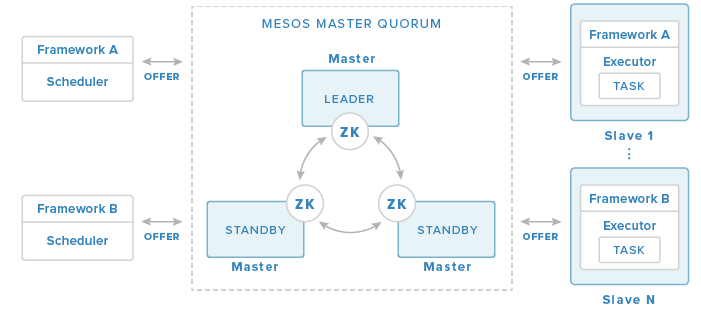
\includegraphics [scale=0.65]{chapitre3/assets/mesosarch.png}
\caption{Architecture de Mesos}
\end{figure}
\begin{itemize}
\item \textbf{Master daemon} : il tourne dans noeud "master" et gère les esclaves.
\item \textbf{Slave daemon} : il tourne aussi dans un noeud "master" et exécute les tâches des frameworks.
\item \textbf{Framework} : connu aussi par l'application Mesos, il est composé d'un ordonnaceur qui gère les offres d'allocation de ressources, et d'un ou plusieurs exécuteurs qui lancent les tâches sur les esclaves.
\item \textbf{Offer} : c'est une liste des ressources disponibles de la mémoire et du CPU propre à un nœud esclave. Tous les nœuds esclaves envoient des offres pour le maître  et ce dernier les transmet aux frameworks disponibles.
\item  \textbf{Task} : c'est un tâche qui est ordonnancée par un framework et qui est exécutée dans un nœud esclave. Cette tâche peut être de n'importe quel type (commande, script bash ,requête SQL, Hadoop Job, ...)
\item \textbf{Apache ZooKeeper }: C'est un logiciel qui coordonne les nœuds maîtres.
\end{itemize}
\subsection{Frameworks Mesos}
Le framework ou l'application Mesos tient une importante place au sein de l'architecture. Dans cette partie , on présentera deux frameworks importants qui sont \textbf{Marathon} et \textbf{Chronos}.
\begin{figure}[H]
\centering
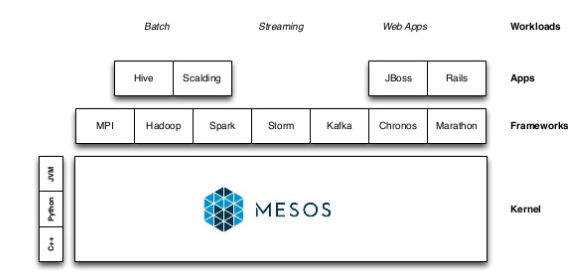
\includegraphics [scale=0.65]{chapitre3/assets/framework.png}
\caption{Composants de l'architecture Mesos}
\end{figure}
\subsubsection*{Marathon}
\emph{Marathon} est un framework Mesos développé pour exécuter les applications "\emph{long-running}". Il sert de remplacement pour le système \emph{init}. Il possède de nombreuses fonctionnalités qui simplifient les applications en cours d'exécution dans un environnement en Cluster telles que la haute disponibilité, les contraintes de nœuds, les contrôles de santé de l'application, une API pour scriptabilité et la découverte de service ainsi qu'un outil facile à utiliser l'interface utilisateur Web UI. Il ajoute ses capacités de mise à l'échelle et d'auto-guérison à l'ensemble des fonctionnalités de Mesos. 
\subsubsection*{Chronos}
\emph{Chronos} est une application Mesos qui a été initialement développé par Airbnb comme remplacement pour le système \emph{cron}.Il est un ordonnanceur pleinement fonctionnel , distribué et tolérant aux pannes pour \emph{Mesos}, ce qui facilite l'orchestration des "\emph{jobs}" qui sont des collections de tâches . Il comprend une API qui permet d'exécuter les scripts de la planification de tâches et une interface web pour la facilité d'utilisation.
\emph{Chronos} est complémentaire à \emph{Marathon} car il fournit une autre façon d'exécuter des applications selon un calendrier ou d'autres conditions telles que la réalisationn d'un autre emploi. Il est également capable de la planification de tâches sur plusieurs nœuds esclaves \emph{Mesos}, et fournit des statistiques sur les échecs et les réussites d'emploi.
\section{Coreos}
\textbf{Coreos} est un système d'exploitation open-source basé sur le noyau \emph{Linux} et construit pour fournir des infrastructures aux déploiements en Cluster. En effet, il est un système minimaliste, sur lequel est greffé des conteneurs applicatifs indépendants et sécurisés. Coreos est conçu pour être léger et performant afin de gérer les datacenters. Coreos consomme 40\% moins de mémoire au démarrage en moyenne par rapport à un serveur \emph{Linux}. Coreos est disponible sur plusieurs plates-formes comme Amazon Compute Cloud, Google Compute Engine et plusieurs autres.
%\begin{figure}[H]
%\centering
%
\includegraphics [scale=0.4]{chapitre3/assets/logocoreos.png}
%\caption{Logo de Coreos}
%\end{figure}
\subsection{Composants de Coreos}
\subsubsection*{Le service Systemd}
\emph{systemd} est une suite de gestion de système, de bibliothèques et utilitaires conçus comme un système central de management et configuration pour le système d'exploitation Linux. Il est contrôlé dans le système d'exploitation Coreos par le service \emph{Fleet}.
\subsubsection*{Le service Etcd}
Le service \emph{etcd} est une base de données distribuée de clé-valeur qui fournit une configuration partagée et un service de découverte pour les Clusters \emph{Coreos}.Il fonctionne sur chaque machine dans un Cluster et gère l'élection du maître lors des partitionnements réseaux ou la perte du maître.
\begin{figure}[H]
\centering
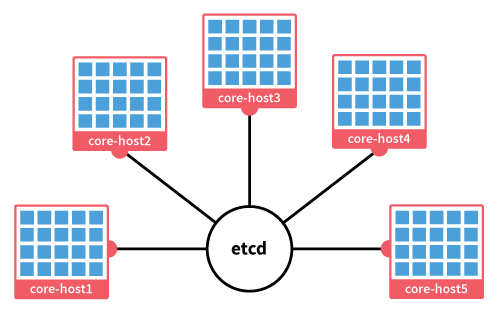
\includegraphics [scale=0.4]{chapitre3/assets/etcd-cluster.png}
\caption{Service etcd.}
\end{figure}
\subsubsection*{Le service Fleet}
\emph{Fleet} permet de traiter le Cluster \emph{Coreos} comme s'il partageait un unique système d'initialisation. Il encourage les utilisateurs à écrire des applications sous forme de petites unités éphémères qui peuvent facilement migrer autour d'un Cluster. En utilisant \emph{Fleet}, les développeurs peuvent se concentrer sur la gestion des conteneurs sans soucier des machines qui tournent les conteneurs. Le service \emph{Fleet} a plusieurs avantages: 
\begin{itemize}
\item Déployer conteneurs docker sur des hôtes arbitraires dans un cluster.
\item Distribuer des services à travers un Cluster à l'aide de niveau machine anti-affinité.
\item Découvrir les machines fonctionnant dans le Cluster.
\item SSH automatiquement dans la machine exécutant un emploi.
\end{itemize}
\begin{figure}[H]
\centering
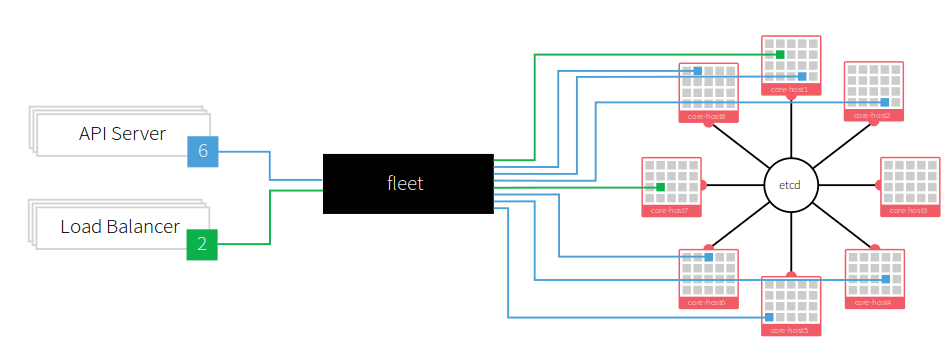
\includegraphics [scale=0.5]{chapitre3/assets/fleet.png}
\caption{Service management Fleet.}
\end{figure}
\end{onehalfspace}


\section{Récapitulation}


\def\arraystretch{1.6}%  1 is the default, change whatever you need

{\rowcolors{1}{tabOdd}{tabEven}
\begin{center}
\begin{table}[H]

	\begin{tabu}{| X[c] | X[c] | X[c] |} 


	\hline
	\rowcolor{tabHead}
	\textbf{CoreOS} & \textbf{Kubernetes} & \textbf{Mesos}\\ [0.95ex] 
	\hline\hline
	Etcd élit le leader du cluster 	& Un master par cluster & Haute disponibilité des masters \\ 
	Orchestration bas niveau & Orchestration haut niveau & Orchestration bas niveau \\ 
	Stable					& Version de pré-production & Stable \\ 
	Rapidité d’installation du cluster & Moins rapide & Moins rapide \\ 
	Bien documenté & Documentation pauvre & Bien documenté \\ 
	Inconscience vis-à-vis les ressources du cluster & Inconscience vis-à-vis les ressources du cluster & Ordonnancement conscient des ressources du cluster \\ 
	Axé sur les conteneurs & Il rassemble des années d’expériences de Google avec l'orchestration des conteneurs	& moins axé sur les conteneurs \\ 
	Destiné pour Docker & Destiné pour Docker	& Utilisé depuis des années pour l'orchestration de Hadoop, il vient de subir un ré-usinage de code pour supporter Docker \\ 
	Limité & Complet (encore plus dans le futur) & Management générique du cluster, extensibilité par les différents ordonnanceurs \\ 
	Pas de proxy et d'équilibreur de charge & Dispose de son propre proxy & Des proxy matures e,enfichables \\ 
	\hline
	\end{tabu}
	\caption{Matrice de décision pour le choix de la solution d'orchestration}
	\label{tab:table_label}

\end{table}
\end{center}
}


Mesos, Kubernetes et CoreOS essaient tous de résoudre des problèmes très similaires, chacun agit dans un niveau d'abstraction. L'on peut imaginer faire des combinaisons les trois solutions d'orchestration en cas de nécessité:

\begin{itemize}
	\item \textbf{CoreOS + Kubernetes}: CoreOS est parfait pour créer rapidement un Cluster. Il va ordonnancer les composants de base de Kubernetes dans le Cluster. L'ordonnancement des conteneurs va être délégué à Kubernetes.
	\item \textbf{Mesos + Kubernetes}: Mesos n'inclut pas nativement un ordonnanceur. L'extensibilité de Mesos fait qu'il est possible de laisser Kubernetes agir comme l'ordonnanceur de Mesos.
	\item \textbf{CoreOS + Mesos + Kubernetes}: L'idée est de jouir de tous les points forts des solutions. En contrepartie, on perd en simplicité, il est préférable de l'adopter qu'en cas de nécessité.
\end{itemize}

Faute de maturité, nous allons adopter CoreOS pour sa stabilité, sa simplicité et sa documentation disponible en dépit qu'il est bas niveau.